\documentclass[11pt,a4paper,titlepage,draft]{article}
\usepackage[utf8]{inputenc}
\usepackage[greek]{babel}
\usepackage{amsmath}
\usepackage{amsfonts}
\usepackage{amssymb}
\usepackage{commath}
\usepackage{xcolor}
\usepackage{hyperref}
\usepackage[skins,theorems]{tcolorbox}
\usepackage{titlesec}

\usetikzlibrary{arrows.meta}

\usepackage[left=2cm,right=2cm,top=2cm,bottom=2cm]{geometry}

\makeatletter
%\newcommand{\attnboxed}[1]{\textcolor{red}{\fbox{\normalcolor\m@th$\displaystyle#1$}}}
\makeatother
\tcbset{highlight math style={enhanced,colframe=red,colback=white,%
  arc=0pt,boxrule=1pt,shrink tight,boxsep=1.5mm,extrude by=0.5mm}}
\newcommand{\attnboxed}[1]{\tcbhighmath[colback=red!5!white,drop fuzzy shadow,arc=0mm]{#1}}
\titleformat{\section}{\bf\Large}{Κεφάλαιο \thesection}{1em}{}
\newtcolorbox{attnbox}[1]{colback=red!5!white,%
  colframe=red!75!black,fonttitle=\bfseries,title=#1}
\newtcolorbox{infobox}[1]{colback=blue!5!white,%
  colframe=blue!75!black,fonttitle=\bfseries,title=#1}


\title{Σημειώσεις Λογισμού ΙΙ}
\date{2016, Εαρινό εξάμηνο}
\author{Καναβούρας Κωνσταντίνος \\ \textlatin{\url{http://users.auth.gr/konkanant}}}



\begin{document}

\maketitle

%\tableofcontents

\newpage

\part{Ατρέας}

\setcounter{section}{-1}

\begin{itemize}
\item 2 ώρες Ζάχαρης (3.5 μον.)
\item 4 ώρες εγώ (6.5 μον.)

\textlatin{http://users.auth.gr/natreas}
\end{itemize}

\paragraph{}

\begin{itemize}
\item Ρασσιάς Θ.
\item Κωνσταντινίδου Μ.
\item Ξένος
\item Σημειώσεις
\end{itemize}

\section[Διανυσματικές συναρτήσεις \& καμπύλες στο χώρο]{Διανυσματικές συναρτήσεις \\ Καμπύλες στο χώρο}

\paragraph{Ορ.}
Μία συνάρτηση \( \mathbf{r}: A \subseteq \mathbb R \rightarrow \mathbb R ^ n \) απαρτίζεται από:

(α). το πεδίο ορισμού της \(A\) που είναι υποσύνολο της πραγματικής ευθείας και

(β). έναν τύπο έτσι ώστε σε κάθε πραγματικό αριθμό \(t \in A\) αντιστοιχεί \textbf{ΜΟΝΑΔΙΚΟ ΔΙΑΝΥΣΜΑ} \( \mathbf{r}(t) \) στο (διανυσματικό) χώρο \( \mathbb R ^ n \) δηλαδή:

\[
A \subseteq \mathbb R \rightarrow \mathbb R ^ n: \mathbf{r}(t) = \left( f_1(t), \dots, f_n(t) \right)
\]

όπου \(f_1: A \subseteq \mathbb R \rightarrow \mathbb R\) \textbf{συνήθεις} πραγματικές συναρτήσεις.

\paragraph{}
Πεδίο ορισμού διανυσματικής συνάρτησης είναι εκείνο το υποσύνολο του \( \mathbb R \) για όλα τα σημεία του οποίου ο τύπος της συνάρτησης \textbf{ΕΧΕΙ ΝΟΗΜΑ}.

\emph{Πρακτικά}, αν
\[ \mathbf{r}(t) = \left( f_1(t), \dots, f_n(t) \right), \]
τότε το πεδίο ορισμού της \( \mathbf{r} \) προκύπτει από τη \textbf{συναλήθευση} των πεδίων ορισμού ΟΛΩΝ των συναρτήσεων \( f_1,\dots,f_n\).

\emph{π.χ.}
\[ \mathbf r (t) = \left( \ln t, \sqrt{1-t^2} \right) 
\quad \leftarrow \text{διανυσματική συνάρτηση πραγματικής μεταβλητής}
\]
Πρέπει
\[
\begin{cases}
t > 0 \text{ (λόγω λογαρίθμου)} \\
\quad \text{και} \\
1-t^2 > 0 \text{ (λόγω ρίζας)}
\end{cases}
\]
Άρα Π.Ο. της \(\mathbf r\) είναι το \((0,1]\).

\subsubsection{Όριο και συνέχεια διανυσματικών συναρτήσεων}
\paragraph{Θ.} Έστω \(\mathbf r: A \subseteq \mathbb R \rightarrow \mathbb R ^ n\), \( \mathbf r(t) =  \left( f_1(t), \dots, f_n(t) \right) \) διανυσματική συνάρτηση και \(t_0\) είναι σημείο συσσώρευσης (σ.σ.) του \(A\).
Τότε:

\[ \lim _{ t \to t_0 } \mathbf r(t) = \vec{a} = \left( a_1, \dots, a_n \right) \iff
\begin{cases}
 \lim_{ t \to t_0 } f_1(t) = a_1 \\
 \quad \vdots \\
 \lim_{ t \to t_0 } f_n(t) = a_n \\
\end{cases}
\]

Επίσης, αν \(τ_0 \in A\) είναι και σ.σ. του \(Α\), τότε:

\[ \mathbf r \text{ συνεχής στο } τ_0 \iff
f_1,f_2,\dots,f_n  \text{ συνεχείς στο } τ_0
\]

δηλ.
\[ \lim _{ t \to t_0 } \mathbf r(t) = \mathbf r (t_0) \iff
\begin{cases}
 \lim_{ t \to t_0 } f_1(t) = f_1(t_0) \\
 \quad \vdots \\
 \lim_{ t \to t_0 } f_n(t) = f_n(t_0) \\
\end{cases}
\]

\subsection{Καμπύλες στον \(\mathbb R^n\)}
\paragraph{Ορ.}
Έστω \(α,β \in \mathbb R\) με \(α<β\). Κάθε \textbf{ΣΥΝΕΧΗΣ} διανυσματική συνάρτηση:
\[
\mathbf{\gamma}: \attnboxed{[a,b]}
\rightarrow \mathbb R^n: \mathbf r_\gamma(t) = \left( f_1(t),f_2(t),\dots,f_n(t) \right)
\]
καλείται καμπύλη στο χώρο \( \mathbb R ^n \) (και το γράφημά της καλείται ΙΧΝΟΣ της \(\mathbf \gamma\)).


\begin{tikzpicture}
\draw[gray, thick] (-2.5,-2.5) -- (2.5,2.5);
\node[above right, rotate=45] at (-2.5,-2.5) {\(+\infty\)};
\node[above left, rotate=45] at (2.5,2.5) {\(-\infty\)};

\filldraw[black] (0.5,0.5) circle (2pt) node[anchor=west] {\(a\)};

\def\away{7}

\draw[->] (xyz cs:x=\away) -- (xyz cs:x=\away+2.5);
\draw[->] (xyz cs:y=0,x=\away) -- (xyz cs:y=2.5,x=\away);
\draw[->] (xyz cs:z=0,x=\away) -- (xyz cs:z=5,x=\away);

\draw[-{>[scale=2.5,width=3]}, gray] (0.5,0.5) to [bend left=90] (\away+1,3);

\coordinate (A) at (\away+1,2);
\coordinate (B) at (\away+2,1,-0.5);
\coordinate (C) at (\away+3.5,3.5);

\draw [blue, very thick] plot [smooth, tension=2] coordinates { (A) (B) (C) };

\draw[->, very thick] (\away,0) -- (A) node[anchor=east] {\(\mathbf r(a)\)};
\draw[->, very thick] (\away,0) -- (B) node[anchor=west] {\(\mathbf r(t)\)};
\draw[->, very thick] (\away,0) -- (C) node[anchor=east] {\(\mathbf r(b)\)};

\end{tikzpicture}



\subsubsection*{}

Έστω \( \gamma: [a,b] \rightarrow \mathbb R ^ n \) καμπύλη.
\begin{itemize}
\item Η \(\gamma\) θα καλείται \textbf{ΑΠΛΗ} αν είναι 1-1, δηλ. \( \forall t \in (a,b) \) με \(t_1 \neq t_2 \implies \mathbf r(t_1) \neq \mathbf r(t_2)\) (δηλ. ΔΕΝ αυτοτέμνεται).

\item Η \(\gamma\) καλείται \textbf{ΑΝΟΙΚΤΗ}, αν \[\mathbf r(a) \neq \mathbf r(b),\] αλλιώς \textbf{ΚΛΕΙΣΤΗ}.

\item Όλες οι καμπύλες \(\gamma: [a,b] \rightarrow \mathbb R ^ n\) \[\mathbf r_\gamma(t) = \left( f_1(t),f_2(t),\dots,f_n(t) \right)\] λέμε ότι είναι καμπύλες σε \textbf{ΠΑΡΑΜΕΤΡΙΚΗ} μορφή και οι
\(
\begin{cases}
x_1 = f_1(t) \\
x_2 = f_2(t) \\
\quad \vdots \\
x_n = f_n(t)
\end{cases}
\) καλούνται παραμετρικές εξισώσεις της \(\gamma\).

\item Δύο καμπύλες μπορεί να έχουν το \textbf{ΙΔΙΟ ΙΧΝΟΣ}.
\paragraph{π.χ.}
\begin{alignat*}{2}
&\mathbf r_{\gamma_1}(t) = ( \cos t,  && \sin t )  \quad t \in [0, 2 \pi ) \\
&\mathbf r_{\gamma_2}(t) = ( \cos t, - && \sin t )  \quad t \in [0, 2 \pi )
\end{alignat*}
Δηλαδή το ίχνος είναι το ίδιο ΑΛΛΑ αλλάζει η ΦΟΡΑ ΔΙΑΓΡΑΦΗΣ ή ο προσανατολισμός.

\emph{Έτσι}, σε κάθε καμπύλη \(\gamma\) σε παραμετρική μορφή αντιστοιχεί με φυσικό τρόπο ένας \textbf{ΠΡΟΣΑΝΑΤΟΛΙΣΜΟΣ} (ή ΦΟΡΑ ΔΙΑΓΡΑΦΗΣ), πάντα προς την κατεύθυνση αύξησης των \(\gamma\).

\item Έστω \(\gamma_1: [a,b] \rightarrow \mathbb R^n, \gamma_2: [b,c] \rightarrow \mathbb R^n\) καμπύλες.

Καλώ \textbf{ΑΝΤΙΘΕΤΗ} της \(\gamma_1\), συμβολικά \(- \gamma_1\), την καμπύλη που έχει ίδιο ΙΧΝΟΣ με τη \(\gamma_1\) αλλά \textbf{αντίθετη} φορά διαγραφής.

\[ -{\gamma_1} : [a,b] \rightarrow \mathbb R^n : \mathbf r_{-\gamma_1}(t) - \mathbf r_{\gamma_1}(a+b-t)
\]

\item Αν \(\mathbf r_{\gamma_1}(b) = r_{\gamma_2}(b)\), ορίζω την καμπύλη \( \gamma_1+\gamma_2 \) ως εξής:
\[
\gamma_1+\gamma_2: [a,c] \rightarrow \mathbb R^n:
\mathbf r_{\gamma_1+\gamma_2}(t) =
\begin{cases}
\mathbf r_{\gamma_1}, \quad t \in [a,b] \\
\mathbf r_{\gamma_2}, \quad t \in (b, c]
\end{cases}
\]

\item Έστω \( \phi: [c,d] \rightarrow [a,b] \) \textbf{συνεχής} και γνησίως \textbf{μονότονη} συνάρτηση. Τότε η \textbf{σύνθεση}: \[ \mathbf \gamma_1 \circ \phi: [c, d] \rightarrow \mathbb R ^n \]
είναι καμπύλη που καλείται \textbf{ΙΣΟΔΥΝΑΜΗ} της \(\gamma_1\) και έχει το \textbf{ΙΔΙΟ ΙΧΝΟΣ} με τη \(\gamma_1\).

\item Αν \(\phi\) γν. αύξουσα, τότε η σύνθεση έχει και ίδιο προσανατολισμό, αλλιώς αντίθετο προσανατολισμό σε σχέση με τη \(\gamma_1\).
\end{itemize}

\subsection{Παραδείγματα καμπύλων σε παραμετρική μορφή}
\begin{itemize}
\item Έστω \(A,B \in \mathbb R^n\), το \(\overrightarrow{AB}\) παραμετροποιείται ως:
\begin{align*}
\mathbf r(t) &= (\text{αρχή}) + (\text{πέρας}-\text{αρχή}), \quad \attnboxed{t \in [0,1]} \\
&= (a_1, \dots, a_n) + t \left( (b_1, \dots, b_n) - (a_1, \dots, a_n) \right) \\
&= \left( a_1 + t (b_1 - a_1 ), \dots, a_n + t (b_n - a_n) \right), \quad \attnboxed{t \in [0,1]}
\end{align*}
επειδή για κάθε σημείο \(X \in \overrightarrow{AB}\):
\[
\overrightarrow{OX} = \overrightarrow{OA} + \overrightarrow{AX}
= \overrightarrow{OA} + t \overrightarrow{AB}
\]

\item Κύκλος \( (x-a)^2 + (y-b)^2 = R^2\) στο χώρο \(\mathbb R^2\):
\[\mathbf r(t) = \left( f_1(t), f_2(t) \right), \quad t \in [a,b] \quad \leftarrow \text{ παραμετροποίηση γενικά} \]
\emph{Ειδικότερα}
\[
\mathbf r(t) = \left( a+R \cos t, b+ R \sin t \right), \quad t \in [0, 2 \pi)
\]
με θετική φορά διαγραφής (αντιωρολογιακή).

Ή:
\[
\mathbf r(t) = \left( a+R \cos t, b - R \sin t \right), \quad t \in [0, 2 \pi)
\] με αρνητική φορά διαγραφής.

\item Συνάρτηση \(y=f(x)\) πραγματική όπου \(x \in [a,b]\)
\[\mathbf r(t) = \left( x(t), y(t) \right), \quad t \in [a,b] \quad \leftarrow \text{ παραμετροποίηση γενικά} \]
\emph{Ειδικότερα}
\[
\mathbf r(t) = \left( t, f(t) \right) \quad t \in [a, b)
\]

\item Έλλειψη \( \left( \frac{x-a}{A} \right) ^ 2 + \left( \frac{y-b}{B} \right) ^ 2 = 1 \quad \left( \mathbb R^2 \right) \)

\[
\begin{cases}
\frac{x-a}{A} &= \cos t \\
\frac{y-b}{B} &= \sin t
\end{cases}, \text{ τότε}
\begin{cases}
\frac{x}{A} = a+ A \cos{t} \\
\frac{y}{B} = b+ B \sin{t}
\end{cases}
\]
Έτσι \(\mathbf r (t) = (x, y) = (a + A \cos t, b + B \sin t), \quad t \in [0, 2 \pi) \) 

\item Υπερβολή \( \left( \frac{x-a}{A} \right) ^ 2 - \left( \frac{y-b}{B} \right) ^ 2 = 1 \quad \left( \mathbb R^2 \right) \)

\[
\mathbf r (t) = (a + A \cosh t, b + B \sinh t), \quad t \in [0, 2 \pi)
\]

\end{itemize}

\subsection{Παράγωγος διανυσματικών συναρτήσεων μίας μεταβλητής}
\paragraph{Ορ.}
Έστω \(\mathbf r: A \subset \mathbb R \rightarrow  \mathbb R^n : \mathbf r(t) = \left( f_1(t), \dots, f_n(t) \right), \quad t_0 \in A \) είναι σ.σ. του \(Α\). Θα λέμε ότι η \(\mathbf r\) παραγωγίσιμη στο \(t_0\) αν υπάρχει το όριο:
\[
\lim _{t \to t_0} \frac{\mathbf r(t)- \mathbf{r}(t_0)}{t-t_0}
\]
ή ισοδύναμα
\[
\lim _{h \to 0} \frac{\mathbf r(t_0+h)- \mathbf{r}(t_0)}{h}
\]
το οποίο είναι \textbf{ΔΙΑΝΥΣΜΑ} που συμβολίζουμε με \(\mathbf r' (t_0)\) ή \(\frac{\dif \mathbf r}{\dif t}\).

\begin{itemize}
\item Αν η \(\mathbf r\) παραγωγίσιμη σε κάθε σημείο του \(Α\), λέμε ότι είναι παραγωγίσιμη στο \(Α\).
\end{itemize}


\paragraph{Θ.}
\(\mathbf{r}\text{ παραγωγίσιμη στο }A \iff f_1,\dots,f_n \text{ παραγ. στο } A\) και
\[
\mathbf r'(t) = \left( f_1'(t),\dots, f_n'(t) \right)
\]

\subsubsection{Γεωμετρική ερμηνεία}
Έστω \(h > 0\)

\begin{tikzpicture}
\draw[gray, thick] (-2.5,-2.5) -- (2.5,2.5);
\node[above right, rotate=45] at (-2.5,-2.5) {\(+\infty\)};
\node[above left, rotate=45] at (2.5,2.5) {\(-\infty\)};

\filldraw[black] (0.5,0.5) circle (2pt) node[anchor=west] {\(t_0\)};
\filldraw[black] (-1,-1) circle (2pt) node[anchor=west] {\(t_0+h\)};


\def\away{7}

\draw[->] (xyz cs:x=\away) -- (xyz cs:x=\away+2.5);
\draw[->] (xyz cs:y=0,x=\away) -- (xyz cs:y=2.5,x=\away);
\draw[->] (xyz cs:z=0,x=\away) -- (xyz cs:z=5,x=\away);

\draw[-{>[scale=2.5,width=3]}, gray] (0.5,0.5) to [bend left=90] (\away+1,3);

\coordinate (A) at (\away+0.2,1);
\coordinate (B) at (\away+1.5,3.2);
\coordinate (C) at (\away+4,4);

\draw [blue, very thick] plot [smooth, tension=1] coordinates { (A) (B) (C) };

%\draw[->, very thick] (\away,0) -- (A) node[anchor=east] {\(\mathbf r(a)\)};
\draw[->, very thick] (\away,0) -- (B) node[anchor=west] {\(\mathbf r(t_0)\)};
\draw[->, very thick] (\away,0) -- (C) node[anchor=east] {\(\mathbf r(t_0+h)\)};

\draw[->] (B) -- (C);


\end{tikzpicture}

Το \( \mathbf r'(t) \) έχει τη διεύθυνση της εφαπτόμενης ευθείας της \( \mathbf r\) στο σημείο \( \mathbf r(τ_0)\) και φορά τη φορά της κίνησης. Μπορεί να αναπαριστά π.χ. την ταχύτητα ενός υλικού σημείου.

\subsubsection{Εξίσωση (Διανυσματική) εφαπτόμενης ευθείας καμπύλης \(\gamma: [a,b] \rightarrow  \mathbb R ^n = \left(f_1(t),\dots,f_n(t) \right)\) παραγωγίσιμης στο σημείο \(t_0\)}

%\small{Αρκεί να ξέρω σημείο της ευθείας και διάνυσμα παράλληλο στην ευθεία}
%TODO
\begin{attnbox}{Προσοχή!!!}
\[
 \mathbf r_{\text{εφ}}(t) =  \mathbf r(t_0) + \lambda \cdot  \mathbf r'(t_0), \quad \lambda \in  \mathbb R 
 \]
 \end{attnbox}
 
\subsubsection{Ιδιότητες παραγώγου}
Έστω \( \mathbf r_1, \mathbf r_2:[a,b] \rightarrow  \mathbb R ^n\) παραγωγ. καμπύλες, τότε:

\begin{itemize}
\item \( \big( \mathbf r_1 \cdot  \mathbf r_2 \big) ' (t) =
 \mathbf r_1' \cdot  \mathbf r_2(t) +  \mathbf r_1 \cdot  \mathbf r_2'(t)
 \) %TODO \cdot εσωτερικό
\item \( \big( \mathbf r_1 \cdot  \mathbf r_2 \big) ' (t) =
 \mathbf r_1' \cdot  \mathbf r_2(t) +  \mathbf r_1 \cdot  \mathbf r_2'(t)
 \)
 \item \begin{align*} 
 [ \mathbf r_1, \mathbf r_2, \mathbf r_3 ]'(t) = 
 &[ \mathbf r_1', \mathbf r_2, \mathbf r_3 ] + \\
 &[ \mathbf r_1, \mathbf r_2',\mathbf r_3 ] + \\
 &[ \mathbf r_1, \mathbf r_2, \mathbf r_3' ]
\end{align*}
\end{itemize}

\part{Ζάχαρης}


\[P = (x_1,\dots,x_n)  \mathbb \quad R ^n\]
\[A = (a_1,\dots,a_n)  \mathbb \quad R ^n\]
\[B = (b_1,\dots,b_n)  \mathbb \quad R ^n\]

\begin{align*}
d(A,B) = &\norm{\overrightarrow{AB}} = \sqrt{(a_1-b_1)^2 + \dots + (a_n-b_n)^2} \\
&\norm{\overrightarrow{OA}} = \sqrt{(a_1)^2 + \dots + (a_n)^2} \\
&\norm{\overrightarrow{OA}} = \sqrt{(b_1)^2 + \dots + (b_n)^2}
\end{align*}

\paragraph{Περιοχή σημείου \(Α\) ακτίνας \(\epsilon\) \(\Pi_\epsilon(A)\)}
\[
\Pi_\epsilon(A) = \left\lbrace P \in  \mathbb R ^n : d(P,A) < \epsilon \right\rbrace
\]
%TODO σχήμα

\paragraph{Σημείο συσσώρευσης}

%\begin{tikzpicture}
%\draw [blue, very thick] plot [smooth, tension=1] coordinates { (0,-2) (1,0) (1,1) (0,-2) };
%\end{tikzpicture}
%TODO

\( E = (E' - \lbrace K\rbrace ) \cup \lbrace I\rbrace \)

\begin{itemize}
\item Σημείο συσσώρευσης: \( \left( \Pi_\epsilon(P) - \left\lbrace P \right\rbrace \right) \cap E \neq \emptyset \)
\item Παράγωγο σύνολο: \(Ε'\) (τα σημεία συσσώρευσης του \(Ε\))
\item Κλειστότητα του \(Ε\): \(Ε \cup E'\)
\item Συνοριακό σημείο \(Α\): \(\forall \epsilon > 0: \Pi_\epsilon(A) \cap E \neq \emptyset\) και \(\Pi_\epsilon(A) \cap \left( \mathbb R^n - E \right) \neq \emptyset\) (το \(Ε\) αλλά και το συμπληρωματικό του ανήκουν σε κάθε περιοχή του \(Α\)).
\item Κλειστό σύνολο: Συμπεριλαμβάνει το σύνορο
\item Ανοικτό σύνολο: Δεν συμπεριλαμβάνει κανένα συνοριακό σημείο
\item Οι χώροι \(\emptyset\) και \( \mathbb R ^ n \) θεωρούνται κλειστοί και ανοικτοί.
\end{itemize}

\paragraph{Συνεκτικό σύνολο (ή συναφές)}
Κάθε δύο σημεία του συνόλου μπορούν να ενωθούν με μια γραμμή που ανήκει στο σύνολο.
%TODO Graph 5

\paragraph{Κυρτό σύνολο}
Κάθε δύο σημεία του συνόλου μπορούν να ενωθούν με \textit{ευθεία} γραμμή που ανήκει στο σύνολο.
%TODO Graph 6

\paragraph{Απλά συνεκτικό σύνολο}
Κάθε καμπύλη του συνόλου θα ανήκει μέσα στο σύνολο αν τη σφίξω.

\paragraph{}
Η μόνη συσχέτιση που ισχύει είναι η εξής:
\begin{align*}
\text{κυρτό} &\implies \text{συνεκτικό} \\
\text{κυρτό} &\implies \text{απλά συνεκτικό}
\end{align*}

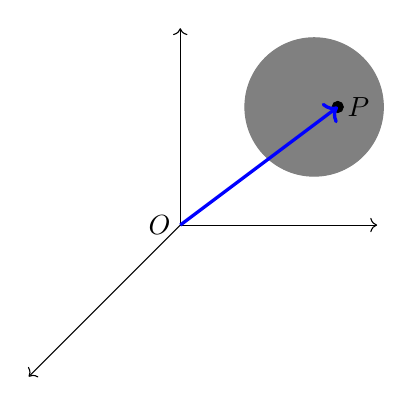
\begin{tikzpicture}
\draw[->] (xyz cs:x=0) -- (xyz cs:x=2.5);
\draw[->] (xyz cs:y=0,x=0) -- (xyz cs:y=2.5,x=0);
\draw[->] (xyz cs:z=0,x=0) -- (xyz cs:z=5,x=0);

\node (0,0) [anchor=east] {\(O\)};

\filldraw[gray] (1.7,1.5) circle (25pt) node[anchor=north] {\(E\)};

\filldraw[black] (2,1.5) circle (2pt) node[anchor=west] {\(P\)};
\draw[->,blue, very thick,anchor=west] (0,0) -- (2,1.5);
\end{tikzpicture}

\paragraph{Φραγμένο σύνολο} ανν \(\norm{\overrightarrow{OP}} = d(O,P)\) πεπερασμένη
\paragraph{Συμπαγές σύνολο} ανν είναι φραγμένο και περιέχει το σύνορο

\subsubsection{Ορισμός συνάρτησης}
\(E \subseteq   \mathbb R^n, \quad B \subseteq  \mathbb R \)
\[f: E \rightarrow B: z = f(x_1, \dots, x_n) \]
\begin{tikzpicture}
%TODO Από κύκλο σε ευθεία
\end{tikzpicture}
\[P = \left( x_1, \dots, x_n \right) \rightarrow \text{πρότυπα ή αρχέτυπα, }z\text{ εικόνες} \]
\begin{tikzpicture}
\draw[->] (xyz cs:x=0) -- (xyz cs:x=2.5);
\draw[->] (xyz cs:y=0,x=0) -- (xyz cs:y=2.5,x=0);
\end{tikzpicture}
\begin{tikzpicture}
\draw[->] (xyz cs:x=0) -- (xyz cs:x=2.5);
\draw[->] (xyz cs:y=0,x=0) -- (xyz cs:y=2.5,x=0);
\draw[->] (xyz cs:z=0,x=0) -- (xyz cs:z=5,x=0);
\end{tikzpicture}
Για συνάρτηση από το \( \mathbb R ^n\), χρειάζομαι \(n+1\) άξονες. Άρα γραφικές παραστάσεις θα κάνουμε για συναρτήσεις το πολύ 2 μεταβλητών, με προοπτική παράσταση ή ισουψείς καμπύλες.

\paragraph{Πολυωνυμική συάρτηση}
Περιέχει όρους της μορφής \(a x_1^{m_1} x_2^{m_2} \cdots x_n^{m_n}, \quad m_1,m_2,\dots,m_n \in  \mathbb N \).

\textit{π.χ.}
\begin{align*}
w&=3x^4y^2z^3+4x^5yz^2-7x^3yz \\
w&=f(x,y,z)
\end{align*}
\[
\mathrm{max} \sum_{i=1}^{n}m_i = \text{βαθμός}(f)
\]

\subparagraph{Ρητή συνάρτηση}
\[
\frac{f(P)}{g(P)} =
\frac{f(x_1,\dots,x_n)}{g(x_1,\dots,x_n)}
\quad
f,g \text{ πολυωνυμικές}
\]

\subsubsection{Όριο συνάρτησης}
\[ \lim_{(x,y) \to (x_0,y_0)} f(x,y) = \lambda\]

\paragraph{Διπλά όρια}
\[ \lim_{x \to x_0} \left( \lim_{y \to y_0} f(x,y) \right), \quad
   \lim_{y \to y_0} \left( \lim_{x \to x_0} f(x,y) \right)
\] 
\begin{attnbox}{}Δεν έχουν απαραίτητα σχέση με το κανονικό όριο (και μπορεί να έχουν διαφορετική τιμή)!
Η ύπαρξη ή/και ισότητα των ορίων δεν είναι διαγνωστική για το όριο της συνάρτησης. Αν υπάρχει το \(\lambda\) και \textbf{υπάρχουν} τα παραπάνω όρια, τότε είναι ίσα με \(\lambda\). Αν τα παραπάνω όρια \textbf{υπάρχουν} και \textbf{δεν} είναι ίσα, τότε το \(\lambda\) \textbf{δεν} υπάρχει.
\end{attnbox}

\begin{tikzpicture}
\draw[->,thick] (0,0) -- (0,4);
\draw[->,thick] (0,0) -- (4,0);

\draw[->,blue] (1,1)--(1,3);
\draw[->,blue] (1,3)--(3,3);

\draw[->,orange] (1,1)--(3,1);
\draw[->,orange] (3,1)--(3,3);

\end{tikzpicture}
\begin{infobox}{Μεθοδολογία}
\begin{align*}
w&=f(x,y) \quad \text{ή}\\
w&=f(x,y,z)
\end{align*}
\[ \lim_{P\to P_0} \]
\begin{enumerate}
\item Επιλέγω για την \(f(x,y)\) μια καμπύλη \(y=g(x)\) του \(Ε\) που περνά από το \(Π_0\) ή \\ επιλέγω για την \(f(x,y,z)\) μια καμπύλη \(y=g(x)\) και \(z=h(x)\) του \(Ε\) που περνά από το \(Π_0\)
\item Αντικαθιστώ και καταλήγω στον υπολογισμό του ορίου \(\lim_{x \to x_0}\)
\item Αν το αποτέλεσμα εξαρτάται από τις παραμέτρους τις καμπύλης, τότε το όριο δεν υπάρχει, ενώ αν δεν εξαρτάται, το αποτέλεσμα είναι μη διαγνωστικό.
\end{enumerate}
\end{infobox}

\begin{infobox}{Μεθοδολογία}
Για ρητές συναρτήσεις \(\frac{f(P)}{g(P}\):
\begin{enumerate}
\item Αν \(B \left[ f(P) \right] > B \left[ g(P) \right]\), μάλλον το όριο υπάρχει.
\item Αν \(B \left[ f(P) \right] \leq B \left[ g(P) \right]\), μάλλον το όριο δεν υπάρχει.
\end{enumerate}
\end{infobox}


\end{document}